\subsection{Results and discussion}

\phantomsection



%%%%%%%%%%%%%%%%
%%% FIGURE 1 %%%
%%%%%%%%%%%%%%%%

\begin{Figure_modified}
  \centering
  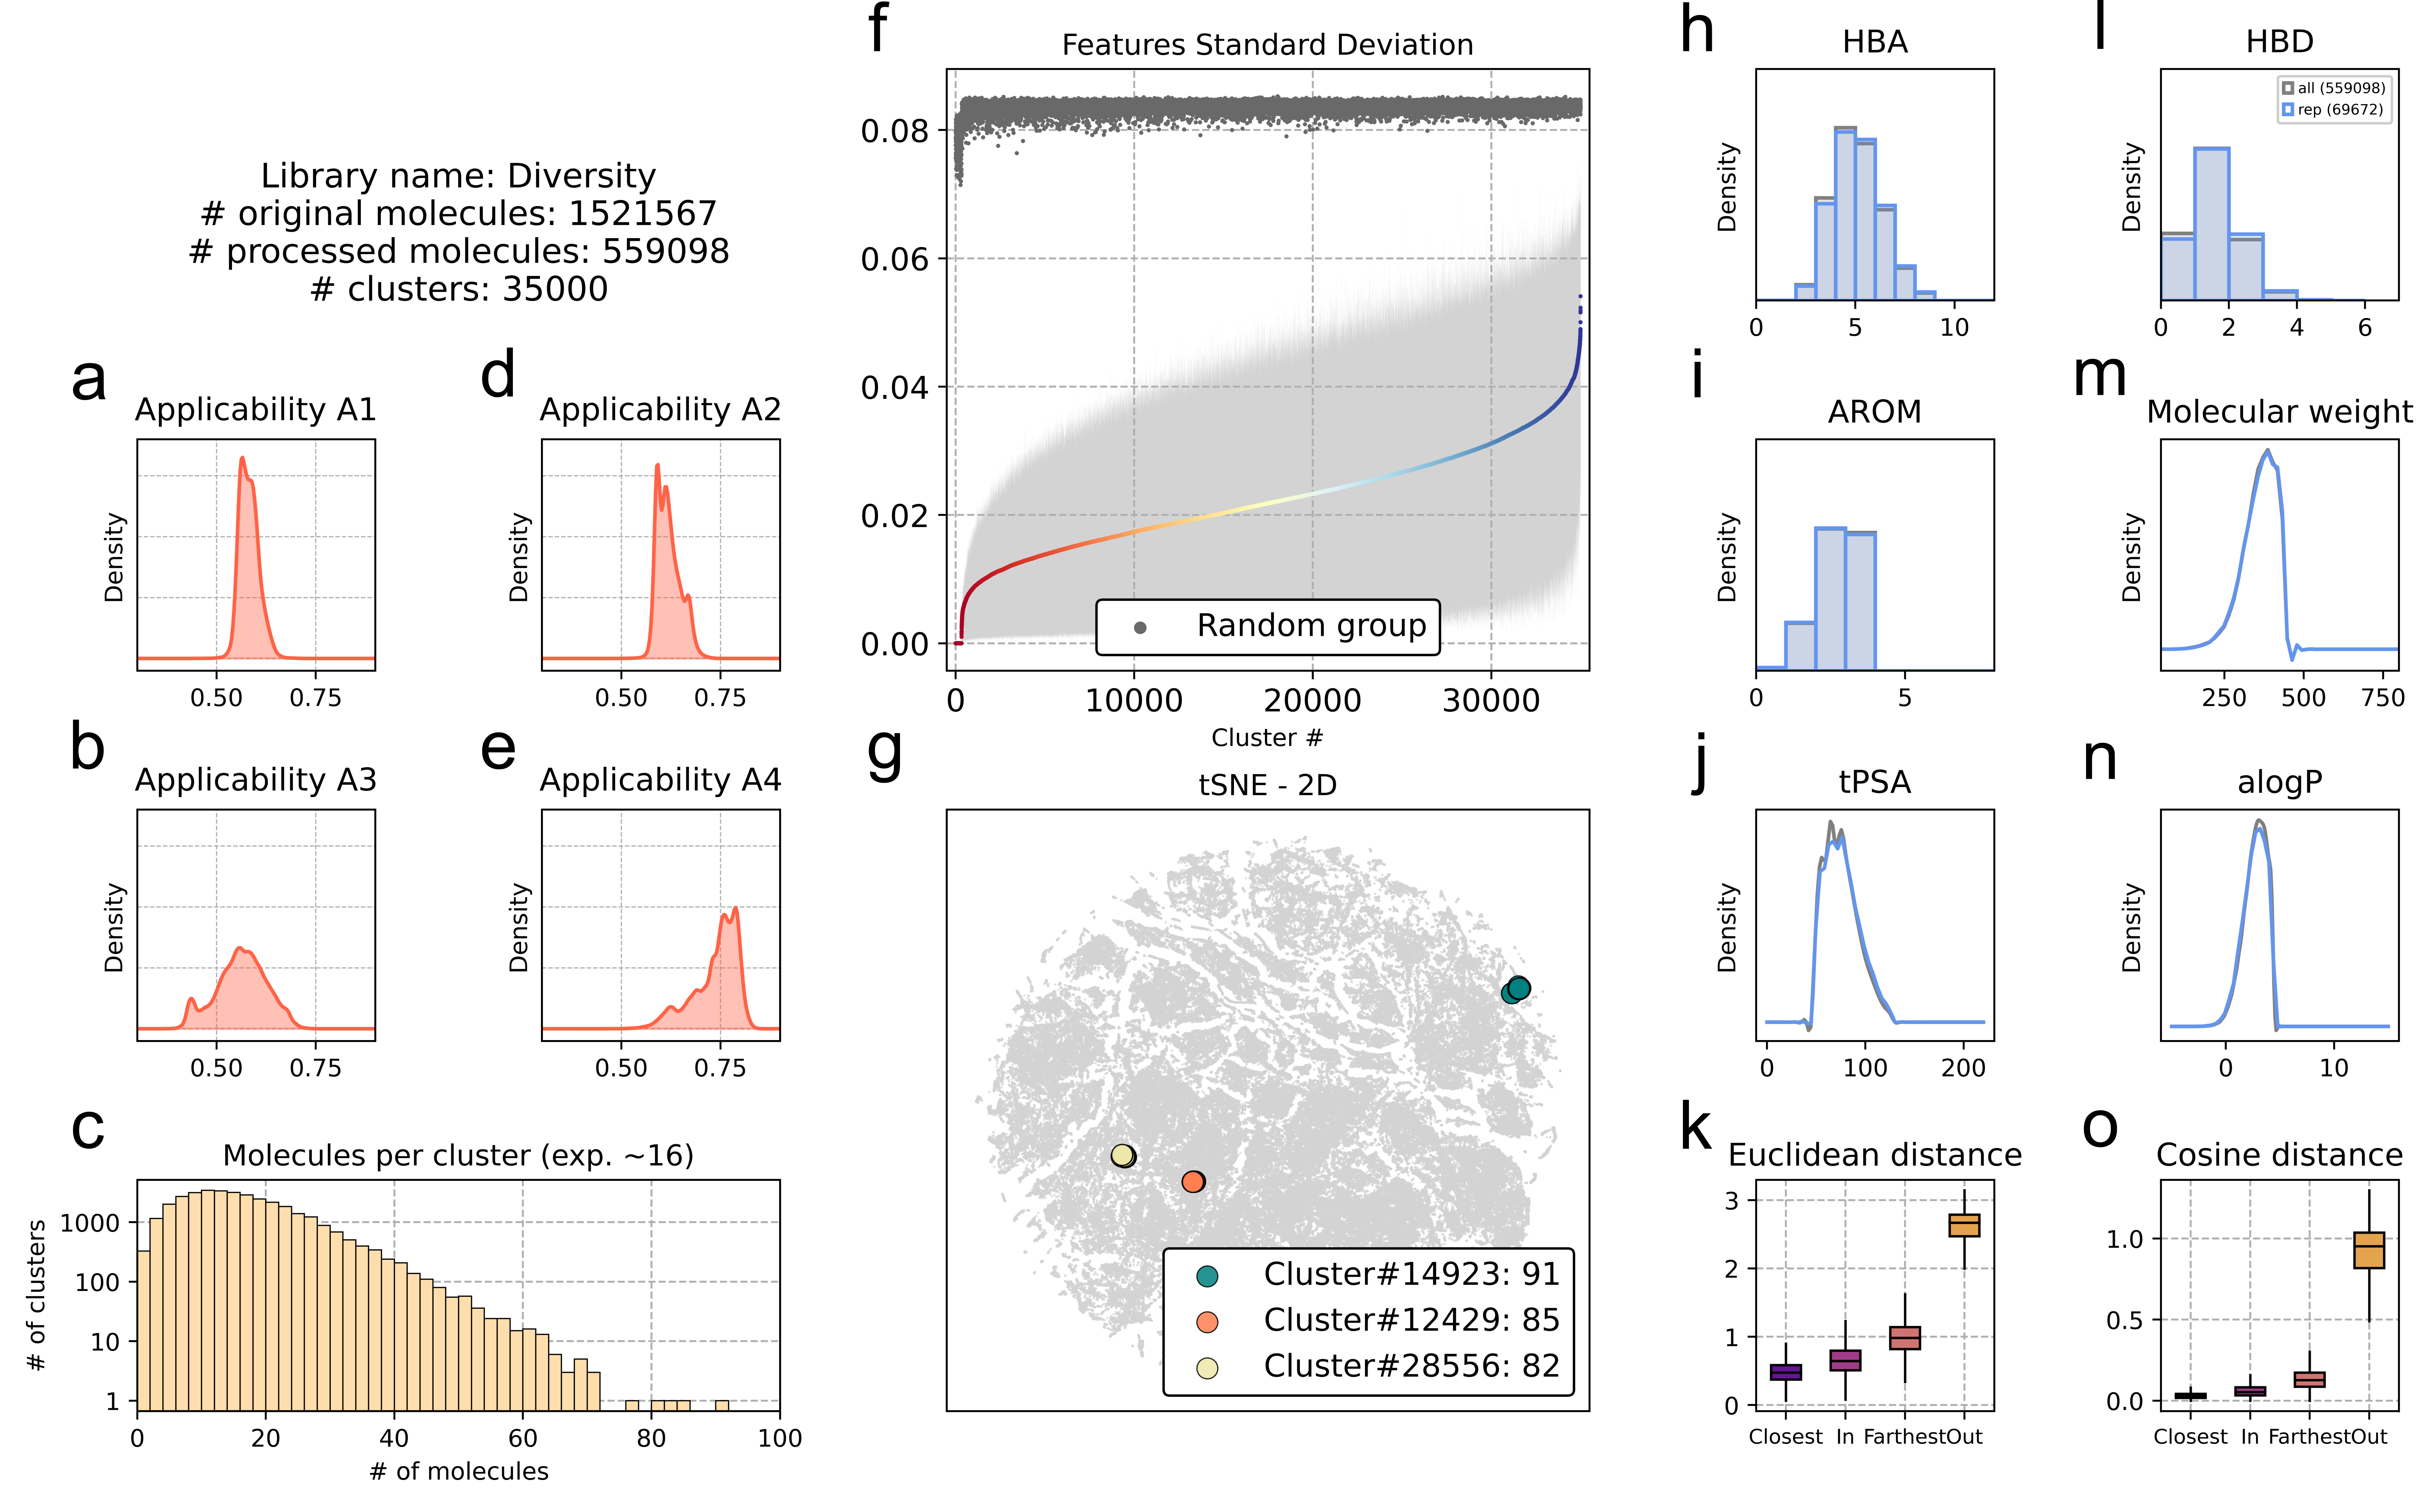
\includegraphics[width=1\linewidth]{figures/Navigation/Main/Diversity_random_v3.png}
  \caption{\textbf{Clustering a chemical library of compounds.}
    \textbf{a,b,d,e)} Distribution of CC signatures’ applicability values for A1, A2, A3 and A4, respectively. 
    \textbf{c)} Number of clusters (y-axis, log scale) having the specified number of molecules (x-axis). The expected number of molecules per cluster is 559k/35k \textasciitilde 16.
    \textbf{f)} For each cluster (x-axis, labeled from 0 to 34,999) standard deviations (y-axis) of the 128 features. Colored points represent the average standard deviation values of the features from signatures within the cluster, light gray bars show the range between the 20\textsuperscript{th} and 80\textsuperscript{th} percentiles of the distribution. Dark gray points represent the average standard deviation values of the features from randomly selected signatures outside the cluster.
    \textbf{g)} 2D tSNE representation of the 559k signaturized compounds (see \hl{Methods}). The top3 most populated clusters are colored accordingly, the legend indicates the number of small molecules within each of these clusters.
    \textbf{h,i,j,l,m,n)} Distributions of number of hydrogen bond acceptors, hydrogen bond donors, aromatic rings, molecular weight, topological polar surface area (tPSA) and alogP for the 559k ChemDiv compounds (after filtering, gray color) and the \textasciitilde70k selected representatives (light blue).
    \textbf{k,o)} Cosine and euclidean distances between the cluster centroid (an abstract 512-dimensional point, see \hl{Methods}) and the nearest compound, the farthest compound and the remaining compounds within each cluster, and a subset of compounds from other clusters.
}
  \vspace{-5mm}
  \rule[0ex]{\textwidth}{0.5pt}
  \vspace{-9mm}
  \label{Navigation_Fig1}
\end{Figure_modified}


%%%%%%%%%%%%%%%%
%%% FIGURE 2 %%%
%%%%%%%%%%%%%%%%

\begin{Figure_modified}
  \centering
  \includegraphics[width=1\linewidth]{figures/Navigation/Main/ALL_PRETTY.png}
  \caption{\textbf{Chemical space visualization of 6 distinct chemical libraries:} Medina, MetaboLights\cite{yurekten_metabolights_2024, haug_metabolights_2019}, CMAUP\cite{hou_cmaup_2024, zeng_cmaup_2019}, Chemical Diversity, RepoHub\cite{corsello_drug_2017} and the Chemical Checker\cite{duran-frigola_extending_2020}. For each combination of small molecule descriptor (A1-A5 and B4 CC Spaces) and compound library, tSNE 2D representation of the 31,052 generated signatures (see \hl{Methods}). Points are colored by density.
}
  \vspace{-5mm}
  \rule[0ex]{\textwidth}{0.5pt}
  \vspace{-9mm}
  \label{Navigation_Fig2}
\end{Figure_modified}

%%%%%%%%%%%%%%%%
%%% FIGURE 3 %%%
%%%%%%%%%%%%%%%%

\begin{Figure_modified}
  \centering
  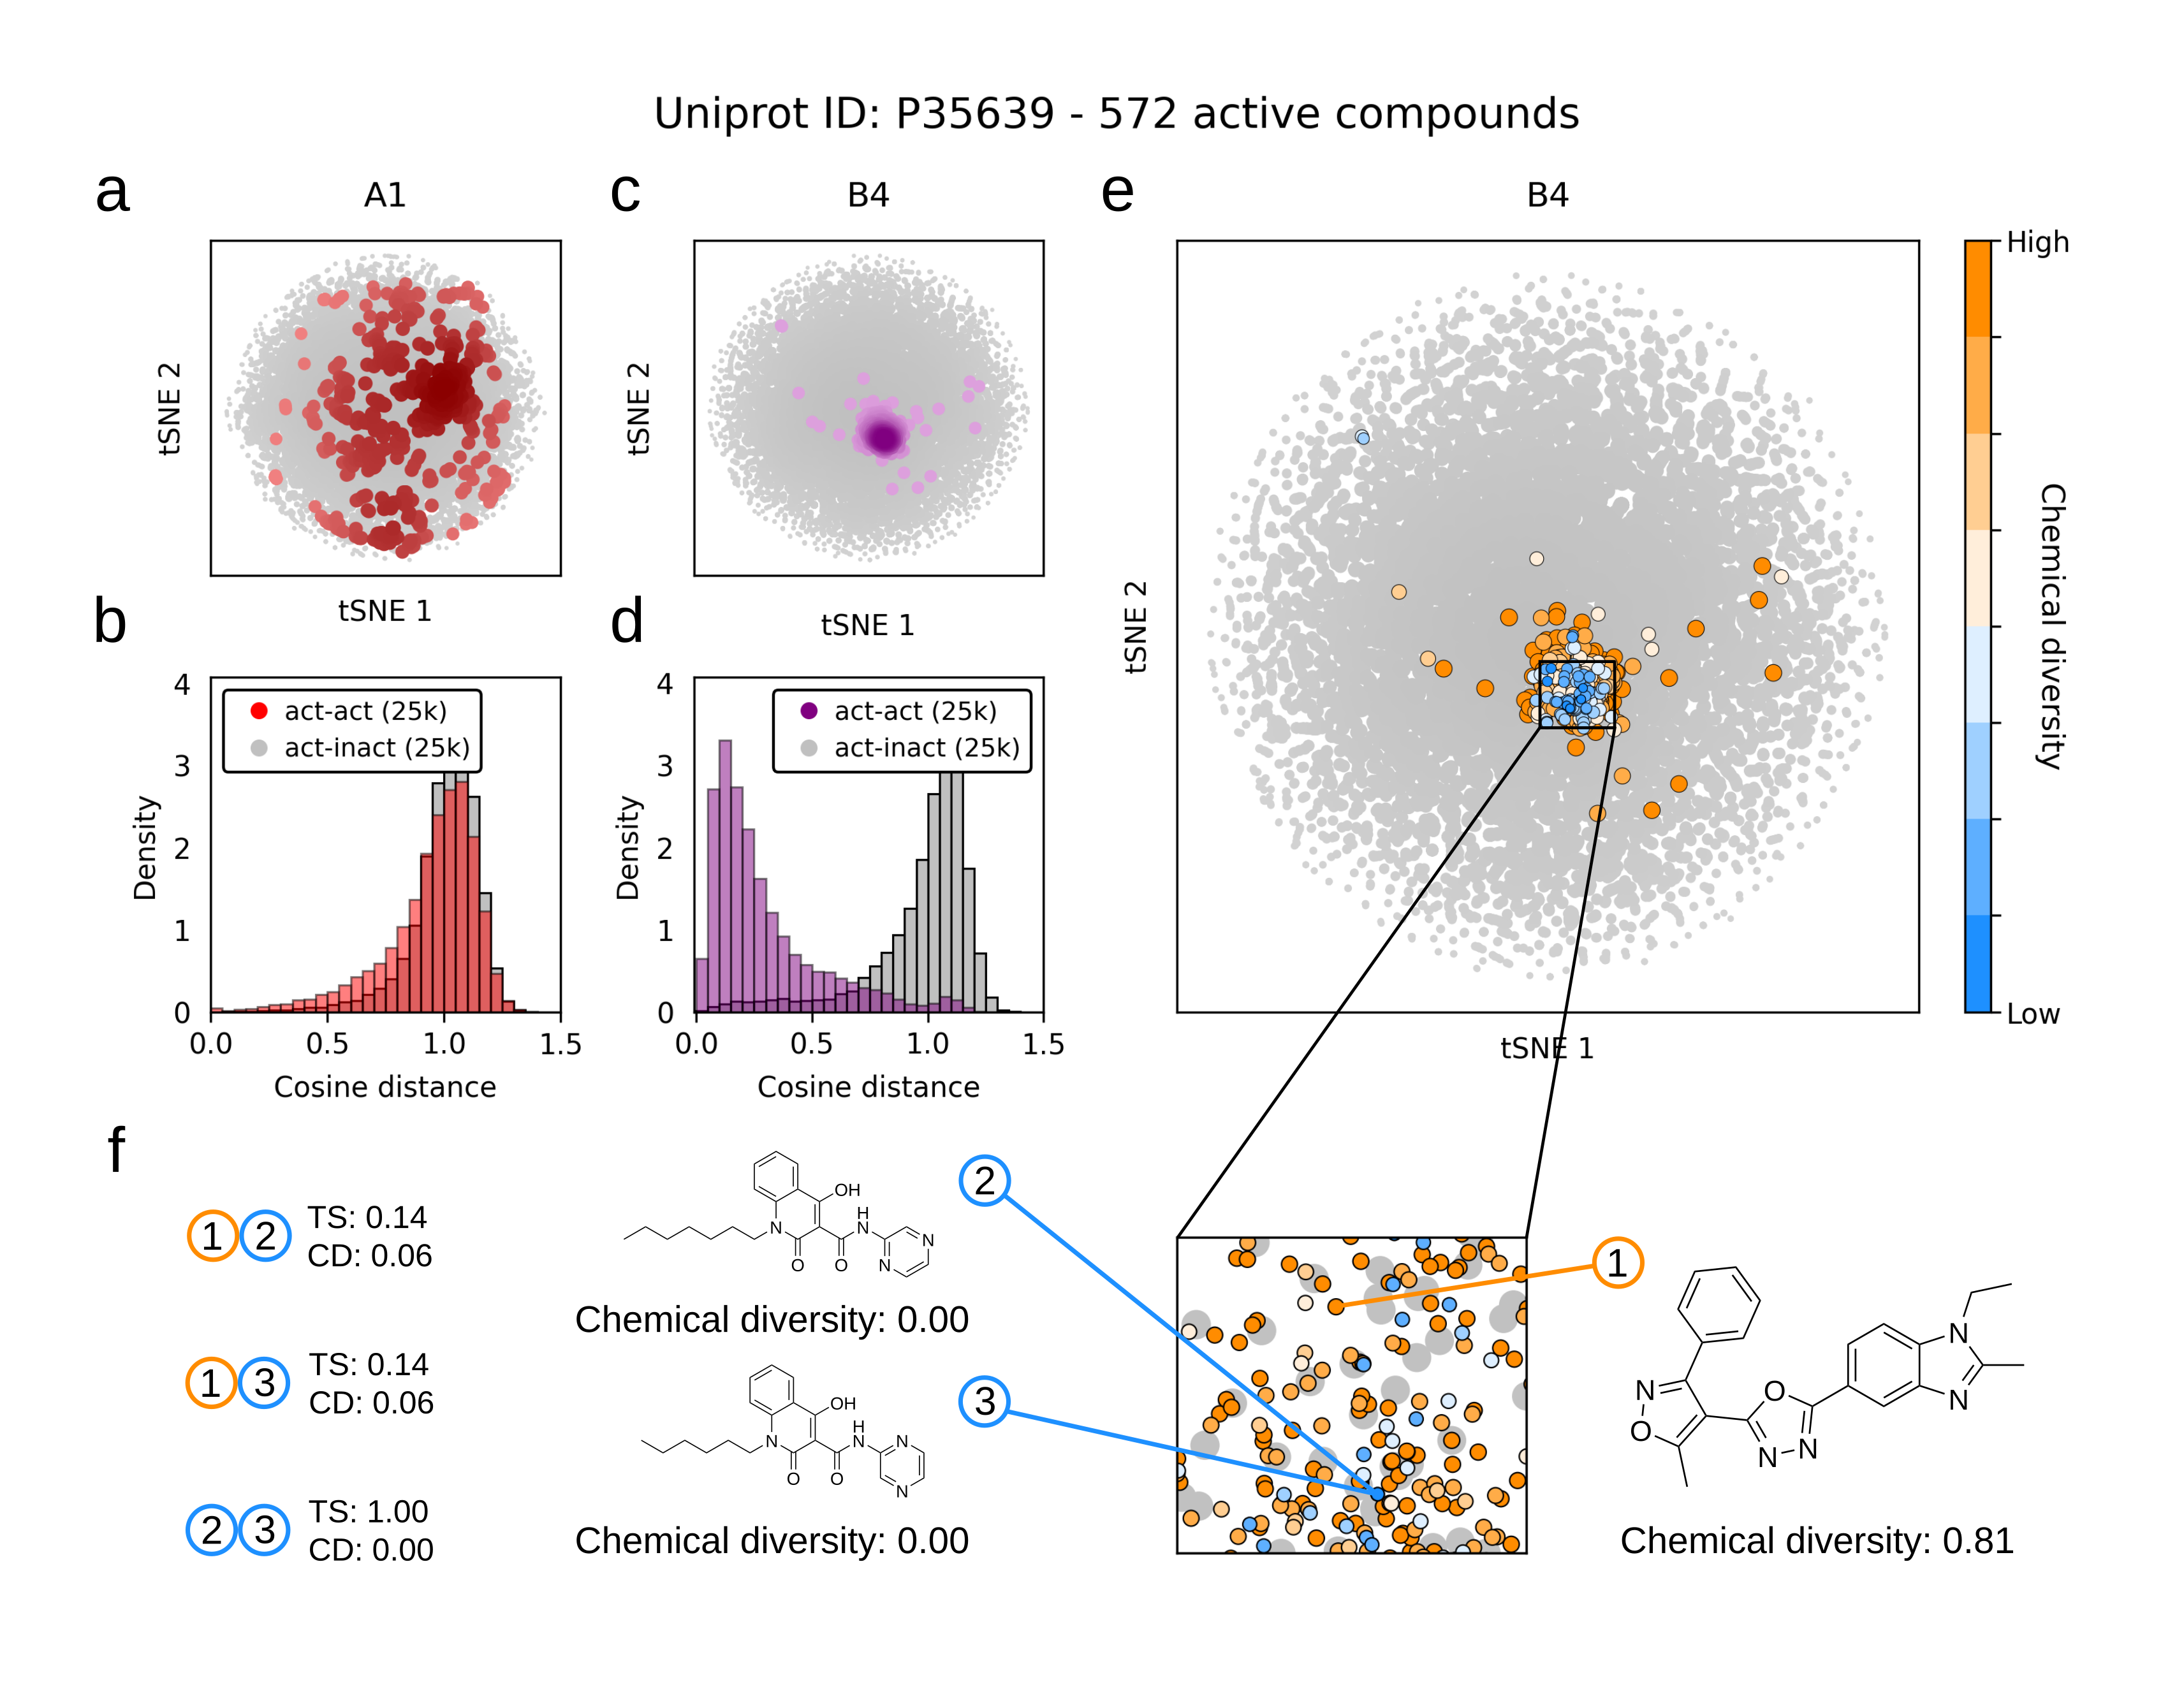
\includegraphics[width=1\linewidth]{figures/Navigation/Main/Fig3_v3.png}
  \caption{\textbf{The advent of bioactivity signatures.}
    \textbf{a)} tSNE 2D representation of the 572 compounds (red, colored by density) reported to be active against P35639 (Uniprot ID, Gene Name: DDIT3) in the CC database (v.2024) derived from ChEMBL and BindingDB. Gray dots correspond to 10k randomly selected compounds that serve as a background of the chemical space. All compounds were previously characterized using the CC A1 signaturizer\cite{bertoni_bioactivity_2021}.
    \textbf{b)} Distribution of cosine distances between active compounds (red, 25k subsampled comparisons) and between active and inactive compounds (gray, 25k subsampled comparisons). All compounds were previously characterized using the CC A1 signaturizer\cite{bertoni_bioactivity_2021}.
    \textbf{c)} tSNE 2D representation of the 572 compounds (purple, colored by density) reported to be active against P35639 (Uniprot ID, Gene Name: DDIT3) in the CC database (v.2024) derived from ChEMBL and BindingDB. Gray dots correspond to 10k randomly selected compounds that serve as a background of the chemical space. All compounds were previously characterized using the CC B4 signaturizer\cite{bertoni_bioactivity_2021}.
    \textbf{d)} Distribution of cosine distances between active compounds (purple, 25k subsampled comparisons) and between active and inactive compounds (gray, 25k subsampled comparisons). All compounds were previously characterized using the CC B4 signaturizer\cite{bertoni_bioactivity_2021}.
    \textbf{e)} tSNE 2D representation of the 572 compounds (colored by chemical diversity, see Methods) reported to be active against P35639 (Uniprot ID, Gene Name: DDIT3) in the CC database (v.2024) derived from ChEMBL and BindingDB. In short, the chemical diversity value represents the chemical redundancy from the neighboring environment of a bioactivity signature. Gray dots correspond to 10k randomly selected compounds that serve as a background of the chemical space. All compounds were previously characterized using the CC B4 signaturizer\cite{bertoni_bioactivity_2021}.
    \textbf{f)} A defined region of the chemical space (see previous subplot) is zoomed in to show (i) a compound having a high chemical diversity value (orange) as well as (ii) a pair of compounds having low chemical diversity (high chemical redundancy, blue). TS: Tanimoto Similarity. CD: Cosine Distance. 
}
  \vspace{-5mm}
  \rule[0ex]{\textwidth}{0.5pt}
  \vspace{-9mm}
  \label{Navigation_Fig3}
\end{Figure_modified}